\chapter{Intensifying competitive pressures} \label{chap3}

\jimi{Need to lead with 'Australian consumers' paying \headline{} too much because of fat, happy non-traded oligopolies. This equates to \$X per household.}

Competition is good for consumers (economic literature): not only lower prices, but better quality products and services, more variety, and potentially greater innovation. There are also benefits for workers: higher wages, greater workplace satisfaction.

But many Australian industries are dominated by a small number of firms. Our two largest companies, Wesfarmers and Woolworths, make more than two-thirds of supermarket revenue. Nearly 80 cents of every dollar loaned in Australia has come from one of the big four banks. And after nearly two decades since it was privatised, Telstra still accounts for nearly half of the revenue in the telecommunications industry, and faces little competition in many rural and regional areas.

Do firms in highly concentrated industries face sufficient competition to keep their margins down and stay innovative? In the US, the evidence suggests that life is too cosy for many incumbent industries -- many firms make persistently high profits without the need for much innovation.

\section{Global worries about growing concentration}



Furman,
The economist



\section{Australia has relatively highly concentrated non-traded sectors; little recent change}

It tends to be high because we are a relatively small economy, dispersed economy, a long way from others. When you have to incur fixed costs to operate in a market, fewer firms find it worthwhile to operate in markets in such economies.

Very high in some sectors; hasn't increased much (\Cref{fig:concentration}). 
Most concentrated sectors include
\begin{itemize}
    \item Retail
    \item Banks
    \item Telco
\end{itemize} 

Traded concentration doesn't matter as much (because you're talking world market shares), and can be net plus if you do have world market share.

\begin{figure}[p] 
 \caption{Concentration is high but hasn't changed much lately}
 \units{Market shares in concentrated industries, 2016}
 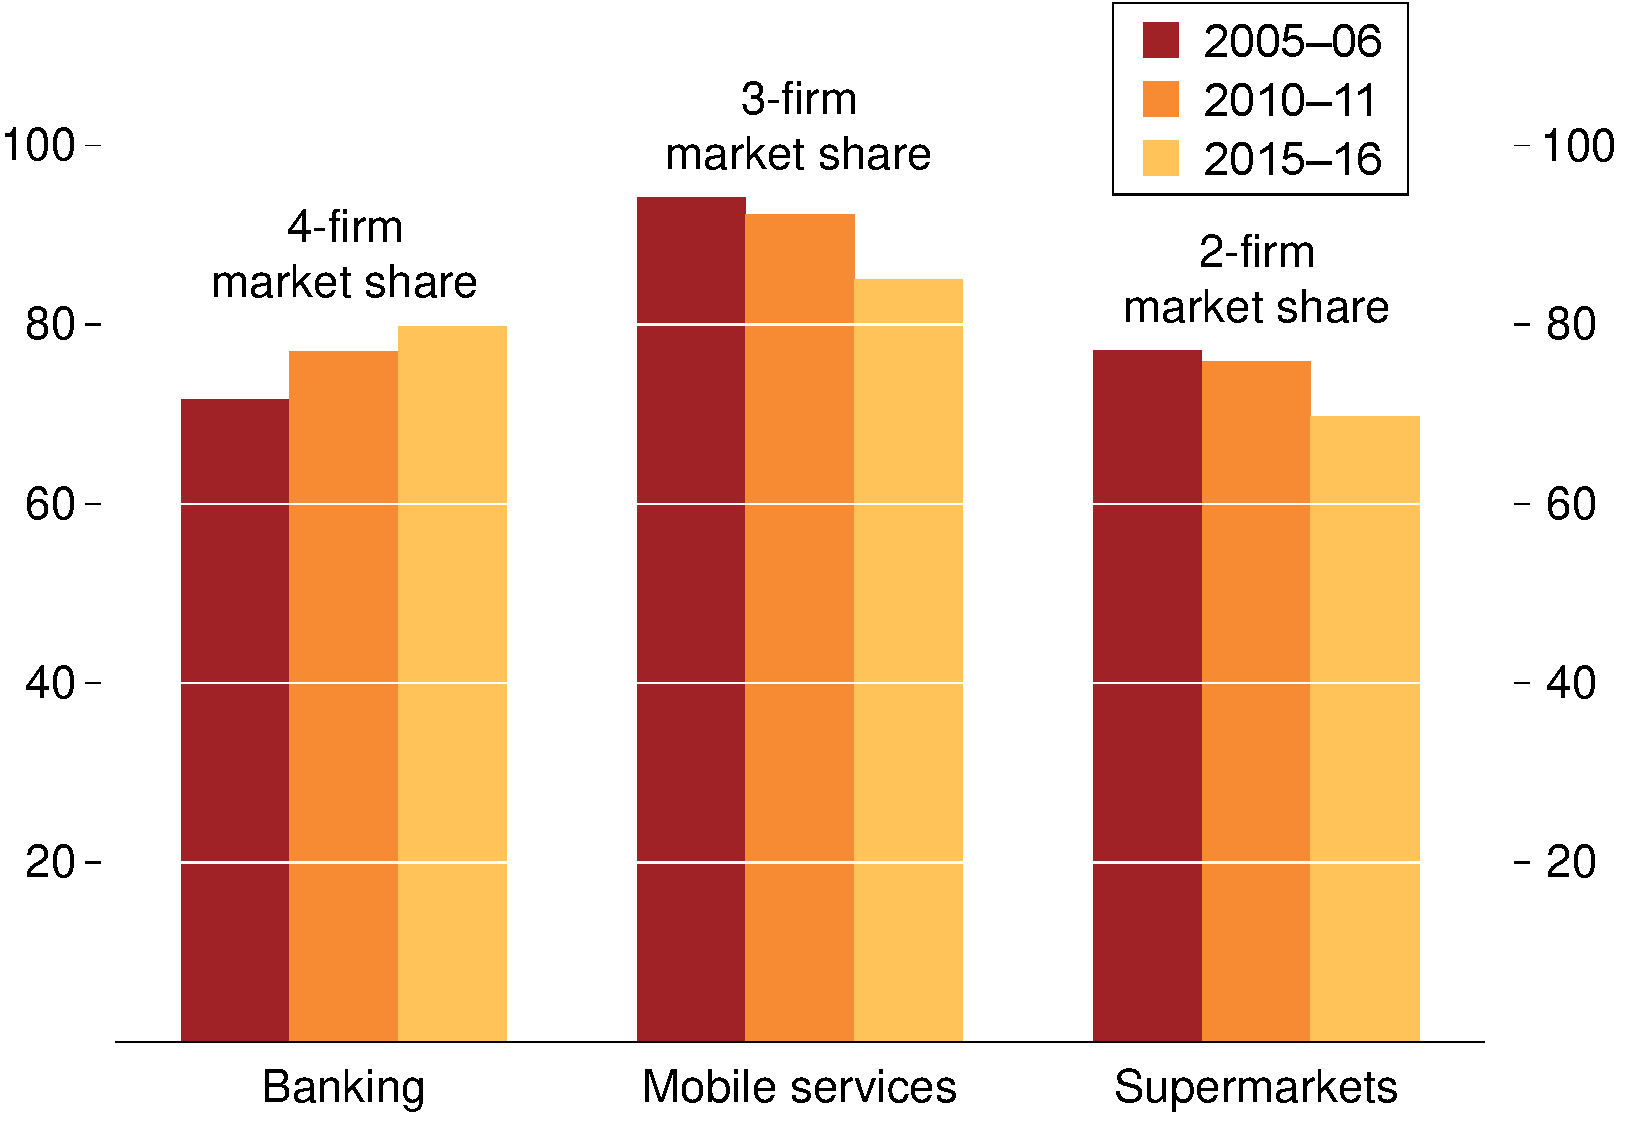
\includegraphics[page=1]{atlas/Change_in_market_share}\label{fig:concentration}
\notes{(PLACEHOLDER)}
\source{Grattan analysis of \textcites{accc2015,apra2016,roymorgan2015,ibisworld2016}.}
\jimi{What share of non-traded GDP?; show it to 2000? APRA: 2003. Size of sectors by revenue or value-added}
\cami{Note: market share measures are not consistent across industries, but consistent within industries. Banking revenue is >\$100k, supermarkets >\$100k, and mobile services probably about \$20--\$30k (but need to confirm) -- so not inconsequential.}
\end{figure}

\section{Concentrated sectors tend to have higher returns}

But that tends to mean the firms face less competitive pressure than they otherwise would.

One way that manifests: ROEs tend to be higher in highly concentrated sectors (\Cref{fig:ROEMargin}). Other studies have found the same thing.  Australia (CIFR study) found that the most concentrated 20 per cent have ROAs that are 5.X percentage points per cent higher than the least concentrated. (any reason to think they appropriate controlled for any confounding factors).\footnote{This relationship is pretty soft -- possibly in part because of the very broad sector definitions used. eg some firms operate in multiple markets but they just get lumped together.}  
\jim{There is no trend in ROE at the level of the whole ASX. Has bumped around in the 8-12 range. May not need a chart}

\begin{figure}[p] 
 \caption{ROES tend to be higher in highly concentrated sectors}
 \units{Average return on equity by GICS industry group, 2011--15, per cent}
 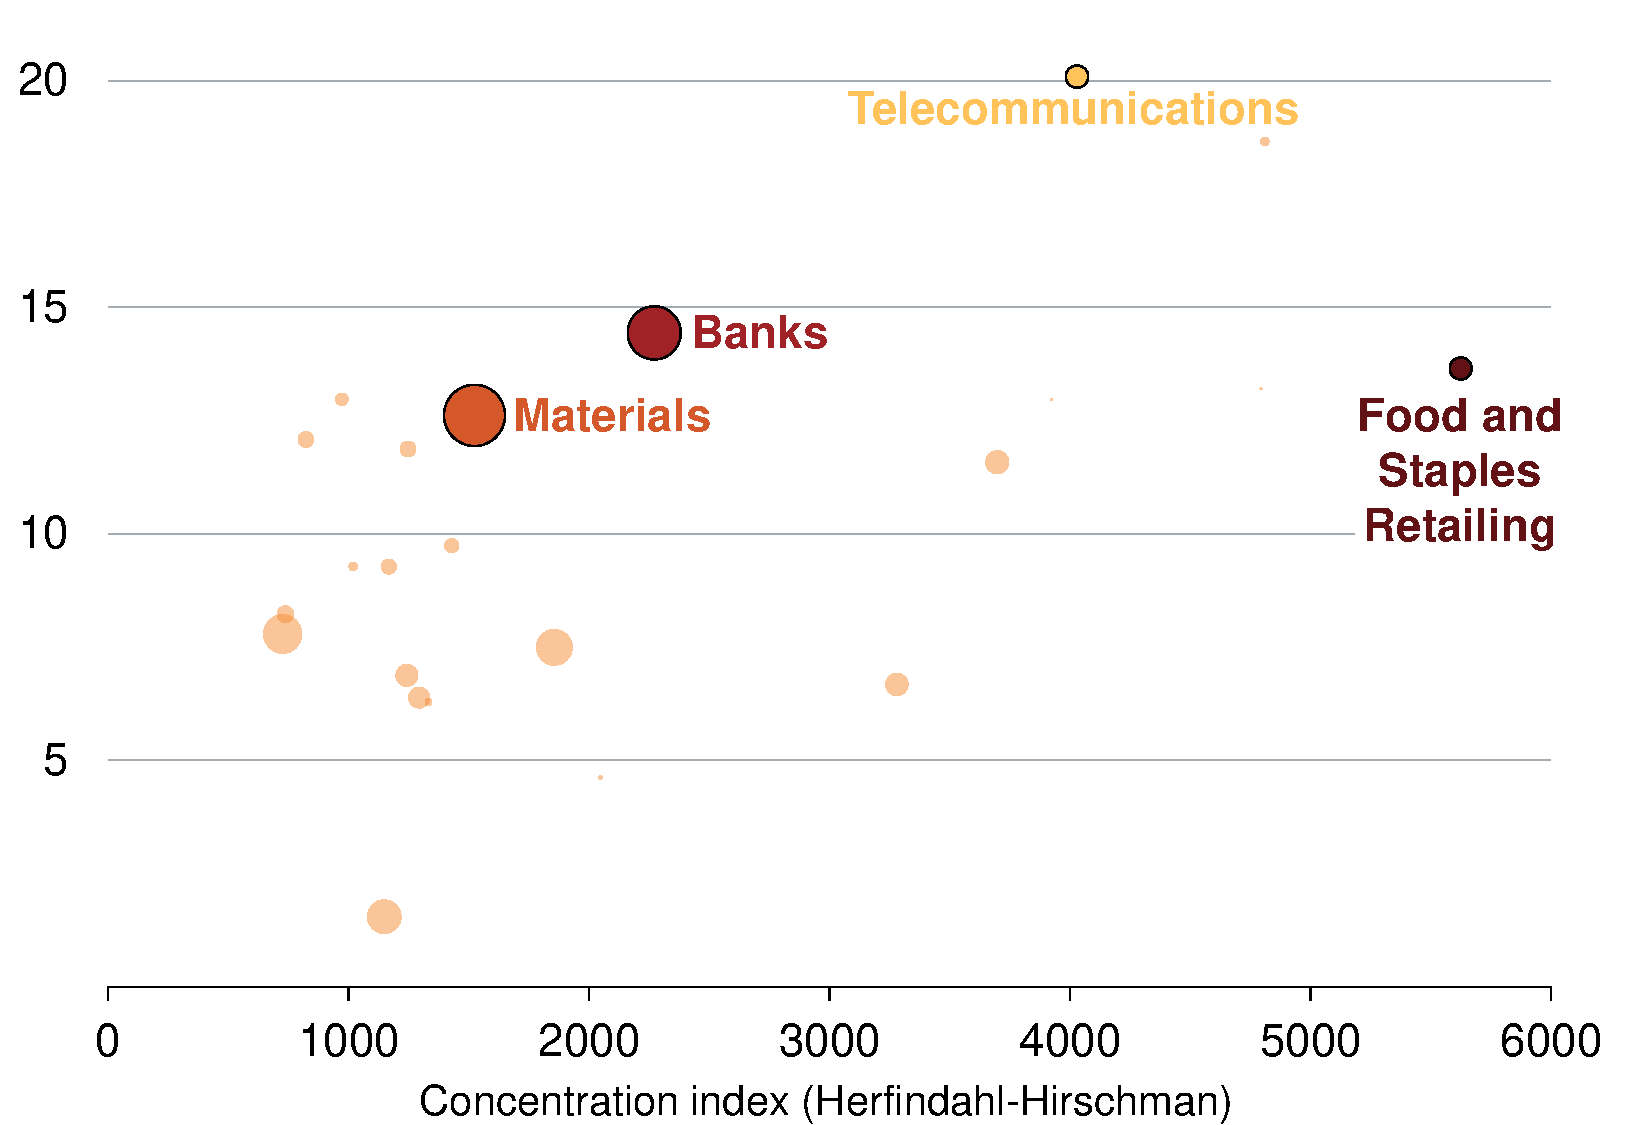
\includegraphics[page=1]{atlas/HH_RoE}\label{fig:ROEMargin}
\notes{Average ROE across five years. Size of bubble corresponds to total equity in industry. Herfindahl-Hirschman index is calculated using firm equity market shares.} 
\source{Grattan analysis of \textcite{morningstar2016}.}
\end{figure}

Suggests margins are higher. Suggests prices are higher. Transfer from consumers, plus efficiency loss. Most high-ROE sectors are:
\begin{itemize}
    \item Retail
    \item Banks
    \item Telco
\end{itemize} 

But this alone is hardly evidence of harm. Could be just economies of scale. 

\begin{figure}[p] 
 \caption{The big four banks have enjoyed a consistently high return on equity}
 \units{Return on equity, big four banks, per cent}
 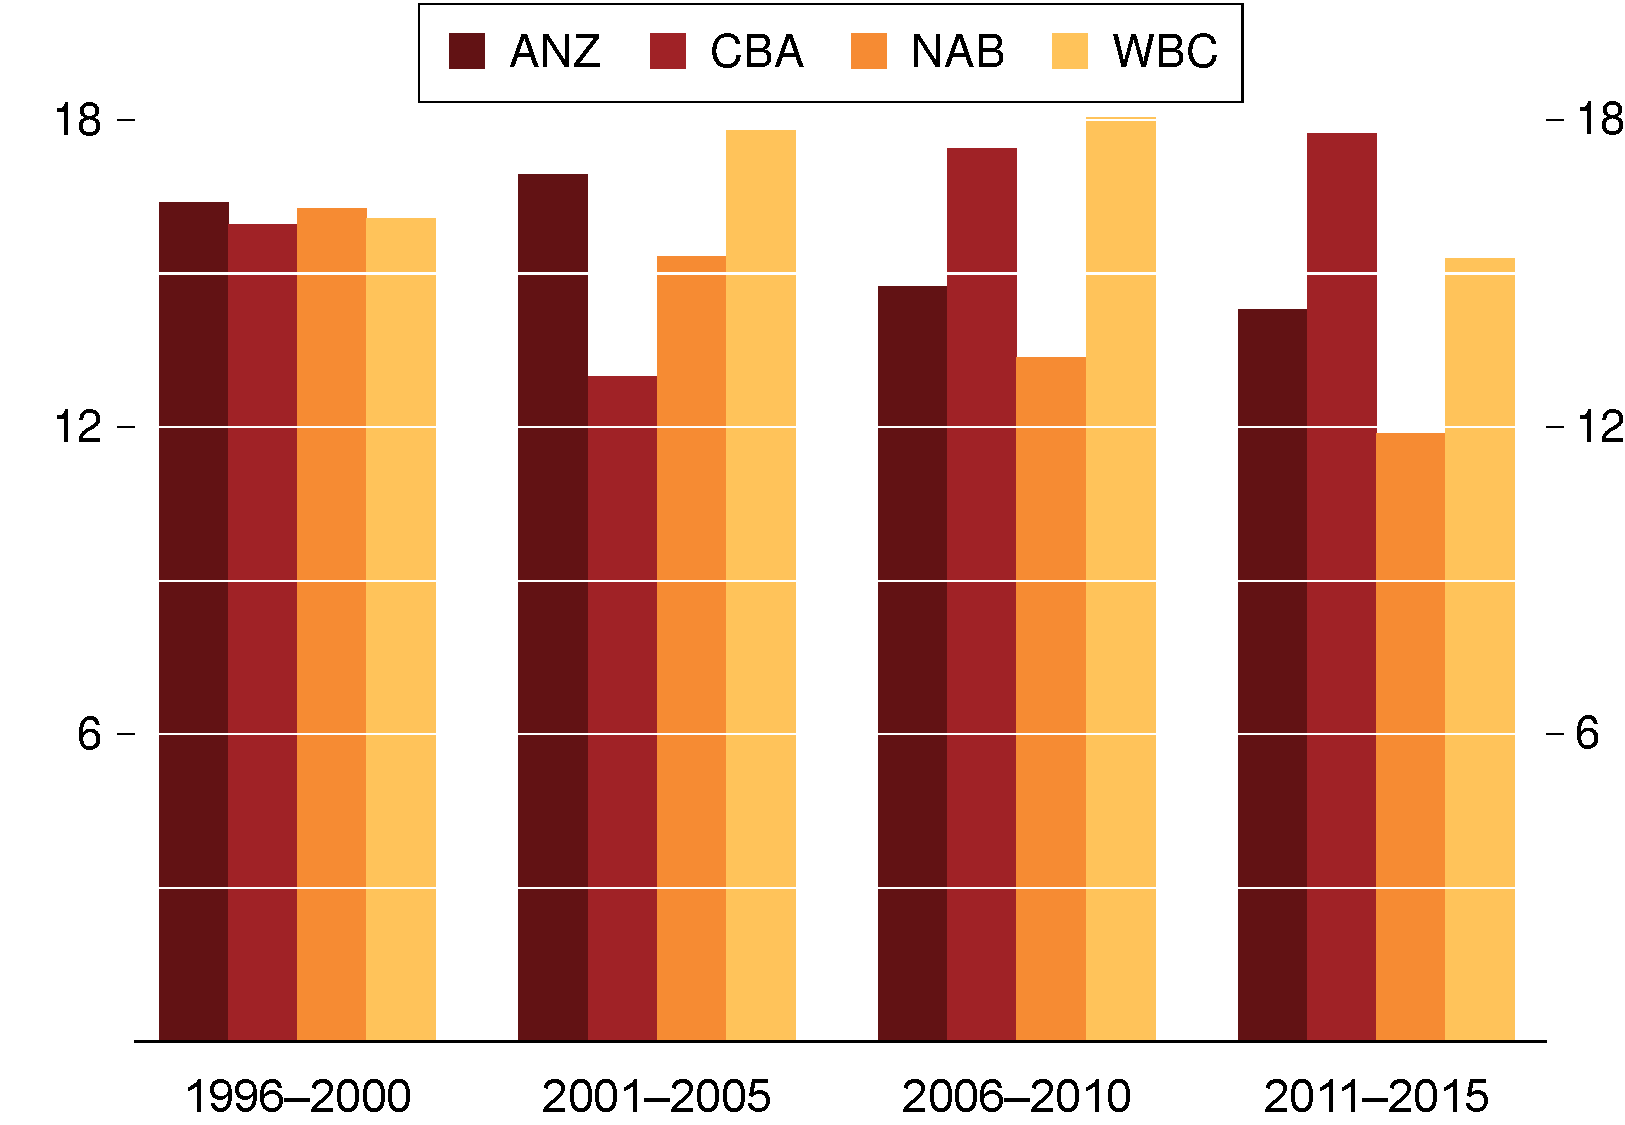
\includegraphics[page=1]{atlas/Banks_ROE}\label{fig:ROE_banks}
\notes{Average ROE across five years.}

\source{Grattan analysis of \textcite{morningstar2016}.}
\end{figure}

\section{Do concentrated sectors have worse service, higher costs, less investment, less innovation}

Lack of competitive pressure means over time they can fall behind
International and Australian evidence suggests that a number of things get worse when firms don't have strong competitive pressure: 
\begin{itemize}
    \item management quality %\jimi{Cam - Treasury speech, Nicholas bloom per Slack} %% CC: resolved
    \begin{itemize}
        \item according to Gruen, the quality of management is highly correlated with productivity -- good management is the efficient use of resources.\footcite{gruen2012productivity}
\cami{We can argue that poor management is a consequence of a lack of competitive pressure, but the real consequence is reduced productivity.}
        \item larger firms typically better managed (and small, family-run firms poorly managed).\footcites{gruen2012productivity,bloom2010management} In highly competitive markets, poorly managed firms are either forced out of the market, or forced to improve to stay in.\footcite{bloom2010management} (results could be driven by either force).
\cami{Of course, the implication of this is that it would be better to have multinationals competing rather than family-run businesses competing -- argument for an optimal number of major players in a given market.}
        \item Australia has a large percentage of very small manufacturing firms, and we perform worse than the US.
        \item Education level of both managers and non-managers correlates with management quality.
        \item International evidence suggests government-owned firms are very badly managed on average (lack of competitive pressure likely to be one factor).\footcite{bloom2010management}
        \item interestingly, well-managed firms also perform better in terms of employee satisfaction, work-life balance etc.\footnote{See \textcite{bloom2010management}, but add reference.} (probably most relevant for knowledge-intensive industries, i.e. where human capital is a key input). So employees may also bear the costs of a lack of competition. 
        \cam{Jim, I seem to recall you saying something about how workers are least satisfied in monopoly industries -- was there a paper that backs this up?}
        \cami{Need to dig deeper, but should be able to produce a relevant chart using the World Management Survey data.}
    \end{itemize}
    \item Service: eg call back. \jim{Is there some Choice service survey or business benchmark we can use and link to industry concentration.}
    \cam{It's possible to download complaints and ombudsman data for various industries via Consumer Affairs. Roy Morgan do a survey, but needs to be purchased (\$2500 per industry report...).}
    \item Cost? (x-inefficiency)
    \item Investment (incentives go both ways)
    \item Innovation: possibly U-shaped? R\&D (patents, copyright, new businesses?)
    \cami{See Aghion et al. paper}

If any of these things get too bad you do have entry. 

\end{itemize} 



\section{What to do to increase competitive pressure}

'Andrew leigh' list:

More or less radical? 

\begin{itemize}
    \item Reduce switching costs. Evidence from mobile number portability suggests it helped.\footnote{\textcite{singer2014consumer} shows that mobile prices fell faster after the introduction of MNC in the US. Would be great to have an Australian source.}
    \item Comparison rates.
    \item Market studies power
    \item Price transparency??? (Not clear if this works as it makes it easier to collude).
    \item "monopoly businesses obliged to create competition"?? \jimi{https://theconversation.com/should-monopoly-businesses-have-an-obligation-to-create-competition-63202}
    \item Rudd bank? (probably not a good idea downside: even worse x-inefficiency; risk management?)
    
\end{itemize} 
